\documentclass[twoside]{book}

% Packages required by doxygen
\usepackage{fixltx2e}
\usepackage{calc}
\usepackage{doxygen}
\usepackage[export]{adjustbox} % also loads graphicx
\usepackage{graphicx}
\usepackage[utf8]{inputenc}
\usepackage{makeidx}
\usepackage{multicol}
\usepackage{multirow}
\PassOptionsToPackage{warn}{textcomp}
\usepackage{textcomp}
\usepackage[nointegrals]{wasysym}
\usepackage[table]{xcolor}

% Font selection
\usepackage[T1]{fontenc}
\usepackage[scaled=.90]{helvet}
\usepackage{courier}
\usepackage{amssymb}
\usepackage{sectsty}
\renewcommand{\familydefault}{\sfdefault}
\allsectionsfont{%
  \fontseries{bc}\selectfont%
  \color{darkgray}%
}
\renewcommand{\DoxyLabelFont}{%
  \fontseries{bc}\selectfont%
  \color{darkgray}%
}
\newcommand{\+}{\discretionary{\mbox{\scriptsize$\hookleftarrow$}}{}{}}

% Page & text layout
\usepackage{geometry}
\geometry{%
  a4paper,%
  top=2.5cm,%
  bottom=2.5cm,%
  left=2.5cm,%
  right=2.5cm%
}
\tolerance=750
\hfuzz=15pt
\hbadness=750
\setlength{\emergencystretch}{15pt}
\setlength{\parindent}{0cm}
\setlength{\parskip}{3ex plus 2ex minus 2ex}
\makeatletter
\renewcommand{\paragraph}{%
  \@startsection{paragraph}{4}{0ex}{-1.0ex}{1.0ex}{%
    \normalfont\normalsize\bfseries\SS@parafont%
  }%
}
\renewcommand{\subparagraph}{%
  \@startsection{subparagraph}{5}{0ex}{-1.0ex}{1.0ex}{%
    \normalfont\normalsize\bfseries\SS@subparafont%
  }%
}
\makeatother

% Headers & footers
\usepackage{fancyhdr}
\pagestyle{fancyplain}
\fancyhead[LE]{\fancyplain{}{\bfseries\thepage}}
\fancyhead[CE]{\fancyplain{}{}}
\fancyhead[RE]{\fancyplain{}{\bfseries\leftmark}}
\fancyhead[LO]{\fancyplain{}{\bfseries\rightmark}}
\fancyhead[CO]{\fancyplain{}{}}
\fancyhead[RO]{\fancyplain{}{\bfseries\thepage}}
\fancyfoot[LE]{\fancyplain{}{}}
\fancyfoot[CE]{\fancyplain{}{}}
\fancyfoot[RE]{\fancyplain{}{\bfseries\scriptsize Generated by Doxygen }}
\fancyfoot[LO]{\fancyplain{}{\bfseries\scriptsize Generated by Doxygen }}
\fancyfoot[CO]{\fancyplain{}{}}
\fancyfoot[RO]{\fancyplain{}{}}
\renewcommand{\footrulewidth}{0.4pt}
\renewcommand{\chaptermark}[1]{%
  \markboth{#1}{}%
}
\renewcommand{\sectionmark}[1]{%
  \markright{\thesection\ #1}%
}

% Indices & bibliography
\usepackage{natbib}
\usepackage[titles]{tocloft}
\setcounter{tocdepth}{3}
\setcounter{secnumdepth}{5}
\makeindex

% Hyperlinks (required, but should be loaded last)
\usepackage{ifpdf}
\ifpdf
  \usepackage[pdftex,pagebackref=true]{hyperref}
\else
  \usepackage[ps2pdf,pagebackref=true]{hyperref}
\fi
\hypersetup{%
  colorlinks=true,%
  linkcolor=blue,%
  citecolor=blue,%
  unicode%
}

% Custom commands
\newcommand{\clearemptydoublepage}{%
  \newpage{\pagestyle{empty}\cleardoublepage}%
}

\usepackage{caption}
\captionsetup{labelsep=space,justification=centering,font={bf},singlelinecheck=off,skip=4pt,position=top}

%===== C O N T E N T S =====

\begin{document}

% Titlepage & ToC
\hypersetup{pageanchor=false,
             bookmarksnumbered=true,
             pdfencoding=unicode
            }
\pagenumbering{alph}
\begin{titlepage}
\vspace*{7cm}
\begin{center}%
{\Large Epic\+Heislab }\\
\vspace*{1cm}
{\large Generated by Doxygen 1.8.13}\\
\end{center}
\end{titlepage}
\clearemptydoublepage
\pagenumbering{roman}
\tableofcontents
\clearemptydoublepage
\pagenumbering{arabic}
\hypersetup{pageanchor=true}

%--- Begin generated contents ---
\chapter{File Index}
\section{File List}
Here is a list of all documented files with brief descriptions\+:\begin{DoxyCompactList}
\item\contentsline{section}{source/driver/{\bfseries con\+\_\+load.\+h} }{\pageref{con__load_8h}}{}
\item\contentsline{section}{source/driver/{\bfseries control\+System.\+c} }{\pageref{controlSystem_8c}}{}
\item\contentsline{section}{source/driver/\hyperlink{controlSystem_8h}{control\+System.\+h} \\*Module that interacts directly with hardware }{\pageref{controlSystem_8h}}{}
\item\contentsline{section}{source/driver/{\bfseries elevio.\+c} }{\pageref{elevio_8c}}{}
\item\contentsline{section}{source/driver/\hyperlink{elevio_8h}{elevio.\+h} \\*Module that contains basic functions for elevator control }{\pageref{elevio_8h}}{}
\item\contentsline{section}{source/driver/{\bfseries logic.\+c} }{\pageref{logic_8c}}{}
\item\contentsline{section}{source/driver/\hyperlink{logic_8h}{logic.\+h} \\*Module that deals with order logic }{\pageref{logic_8h}}{}
\item\contentsline{section}{source/driver/{\bfseries terminal\+Updates.\+c} }{\pageref{terminalUpdates_8c}}{}
\item\contentsline{section}{source/driver/\hyperlink{terminalUpdates_8h}{terminal\+Updates.\+h} \\*Module for printing in terminal }{\pageref{terminalUpdates_8h}}{}
\end{DoxyCompactList}

\chapter{File Documentation}
\hypertarget{controlSystem_8h}{}\section{source/driver/control\+System.h File Reference}
\label{controlSystem_8h}\index{source/driver/control\+System.\+h@{source/driver/control\+System.\+h}}


Module that interacts directly with hardware.  


{\ttfamily \#include \char`\"{}elevio.\+h\char`\"{}}\newline
Include dependency graph for control\+System.\+h\+:
\nopagebreak
\begin{figure}[H]
\begin{center}
\leavevmode
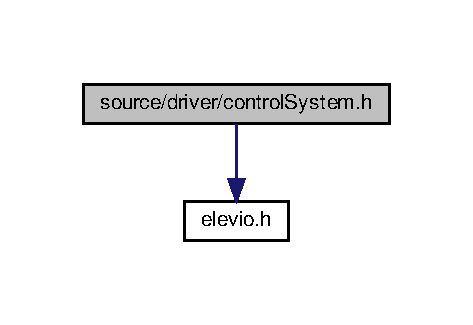
\includegraphics[width=227pt]{controlSystem_8h__incl}
\end{center}
\end{figure}
This graph shows which files directly or indirectly include this file\+:\nopagebreak
\begin{figure}[H]
\begin{center}
\leavevmode
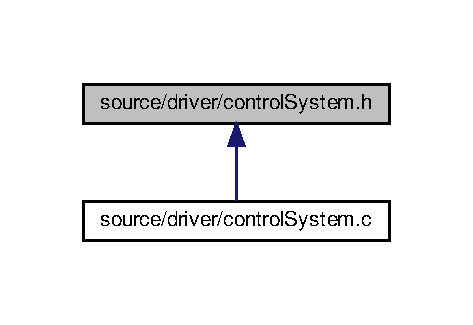
\includegraphics[width=227pt]{controlSystem_8h__dep__incl}
\end{center}
\end{figure}
\subsection*{Functions}
\begin{DoxyCompactItemize}
\item 
\mbox{\Hypertarget{controlSystem_8h_aa58666b14bf8f41a736f9d1dbf3b722b}\label{controlSystem_8h_aa58666b14bf8f41a736f9d1dbf3b722b}} 
void \hyperlink{controlSystem_8h_aa58666b14bf8f41a736f9d1dbf3b722b}{init\+Elev\+Pos} ()
\begin{DoxyCompactList}\small\item\em Initializes elevator by moving it upwards until it reaches a defined floor. \end{DoxyCompactList}\item 
\mbox{\Hypertarget{controlSystem_8h_a1ccddea01ca0b37586eee0448da987ec}\label{controlSystem_8h_a1ccddea01ca0b37586eee0448da987ec}} 
void \hyperlink{controlSystem_8h_a1ccddea01ca0b37586eee0448da987ec}{wait3\+Sec} ()
\begin{DoxyCompactList}\small\item\em System sleeps for 3 seconds. Stop button breaks sleep and exits function. \end{DoxyCompactList}\item 
\mbox{\Hypertarget{controlSystem_8h_a83eae95e057f2236dc2bfa3c0e6575e5}\label{controlSystem_8h_a83eae95e057f2236dc2bfa3c0e6575e5}} 
void \hyperlink{controlSystem_8h_a83eae95e057f2236dc2bfa3c0e6575e5}{check\+Stop\+Button} ()
\begin{DoxyCompactList}\small\item\em Checks if stop button is pressed. If pressed, motor stops. Door opens if elevator is on a defined floor. \end{DoxyCompactList}\item 
\mbox{\Hypertarget{controlSystem_8h_a12abbdcf72325806018fc0ab0cf3abb9}\label{controlSystem_8h_a12abbdcf72325806018fc0ab0cf3abb9}} 
void \hyperlink{controlSystem_8h_a12abbdcf72325806018fc0ab0cf3abb9}{floor\+Indicator\+Light} ()
\begin{DoxyCompactList}\small\item\em Changes floor indicator light if elevator reaches a defined floor. \end{DoxyCompactList}\end{DoxyCompactItemize}


\subsection{Detailed Description}
Module that interacts directly with hardware. 

\begin{DoxyAuthor}{Author}
Christian \& Ida 
\end{DoxyAuthor}
\begin{DoxyVersion}{Version}
0.\+1 
\end{DoxyVersion}
\begin{DoxyDate}{Date}
2022-\/02-\/25 
\end{DoxyDate}

\hypertarget{elevio_8h}{}\section{source/driver/elevio.h File Reference}
\label{elevio_8h}\index{source/driver/elevio.\+h@{source/driver/elevio.\+h}}


Module that contains basic functions for elevator control.  


This graph shows which files directly or indirectly include this file\+:
\nopagebreak
\begin{figure}[H]
\begin{center}
\leavevmode
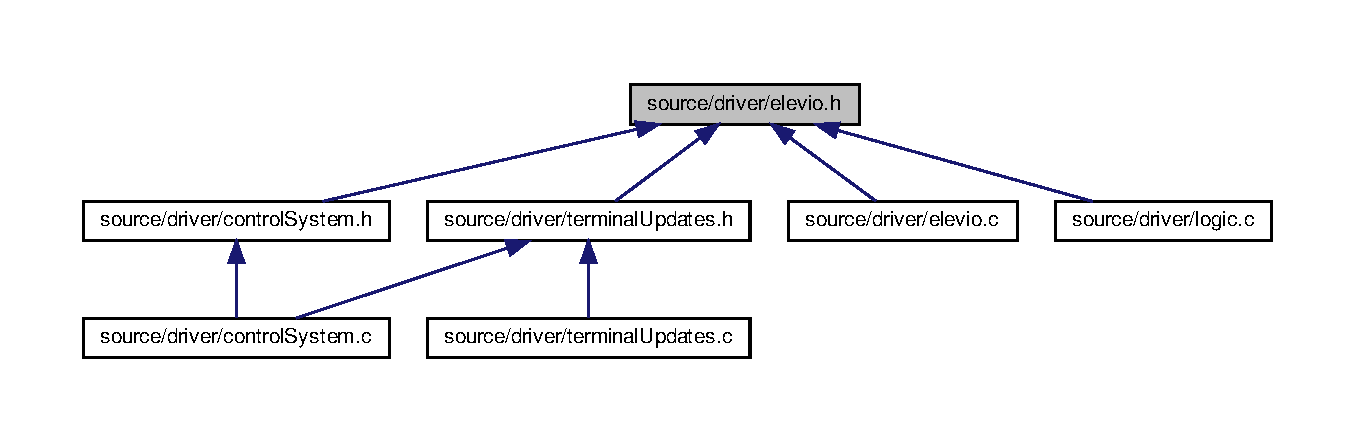
\includegraphics[width=350pt]{elevio_8h__dep__incl}
\end{center}
\end{figure}
\subsection*{Macros}
\begin{DoxyCompactItemize}
\item 
\mbox{\Hypertarget{elevio_8h_ae0592e3739e5e1e76234bb1caf9d1305}\label{elevio_8h_ae0592e3739e5e1e76234bb1caf9d1305}} 
\#define \hyperlink{elevio_8h_ae0592e3739e5e1e76234bb1caf9d1305}{N\+\_\+\+F\+L\+O\+O\+RS}~4
\begin{DoxyCompactList}\small\item\em An enum which represents elevator direction. \end{DoxyCompactList}\item 
\mbox{\Hypertarget{elevio_8h_a271dda243b0f5bd7d2053d258eb71962}\label{elevio_8h_a271dda243b0f5bd7d2053d258eb71962}} 
\#define \hyperlink{elevio_8h_a271dda243b0f5bd7d2053d258eb71962}{N\+\_\+\+B\+U\+T\+T\+O\+NS}~3
\begin{DoxyCompactList}\small\item\em An enum relating buttons for a given floor to numbers. \end{DoxyCompactList}\end{DoxyCompactItemize}
\subsection*{Enumerations}
\begin{DoxyCompactItemize}
\item 
\mbox{\Hypertarget{elevio_8h_ab0dd3595d7049b92115a766f0ea6f7e0}\label{elevio_8h_ab0dd3595d7049b92115a766f0ea6f7e0}} 
enum {\bfseries Motor\+Direction} \{ {\bfseries D\+I\+R\+N\+\_\+\+D\+O\+WN} = -\/1, 
{\bfseries D\+I\+R\+N\+\_\+\+S\+T\+OP} = 0, 
{\bfseries D\+I\+R\+N\+\_\+\+UP} = 1
 \}
\item 
\mbox{\Hypertarget{elevio_8h_ae2d5c50fae96a83cc4f5974af78e6943}\label{elevio_8h_ae2d5c50fae96a83cc4f5974af78e6943}} 
enum {\bfseries Button\+Type} \{ {\bfseries B\+U\+T\+T\+O\+N\+\_\+\+H\+A\+L\+L\+\_\+\+UP} = 0, 
{\bfseries B\+U\+T\+T\+O\+N\+\_\+\+H\+A\+L\+L\+\_\+\+D\+O\+WN} = 1, 
{\bfseries B\+U\+T\+T\+O\+N\+\_\+\+C\+AB} = 2
 \}
\end{DoxyCompactItemize}
\subsection*{Functions}
\begin{DoxyCompactItemize}
\item 
\mbox{\Hypertarget{elevio_8h_acec5e6d14134b881216887fe15aca830}\label{elevio_8h_acec5e6d14134b881216887fe15aca830}} 
void \hyperlink{elevio_8h_acec5e6d14134b881216887fe15aca830}{elevio\+\_\+init} (void)
\begin{DoxyCompactList}\small\item\em Initializes computer connection with elevator hardware and gives out error(s) if it is not able to connect properly. \end{DoxyCompactList}\item 
void \hyperlink{elevio_8h_ab2e6dcf199387c1dd6f78e2bf6fff56e}{elevio\+\_\+motor\+Direction} (Motor\+Direction dirn)
\begin{DoxyCompactList}\small\item\em Sends a direction command to elevator motor. \end{DoxyCompactList}\item 
void \hyperlink{elevio_8h_a182079eb4c29f71ff3b5049a2fd082a3}{elevio\+\_\+button\+Lamp} (int floor, Button\+Type button, int value)
\begin{DoxyCompactList}\small\item\em Sends a on/off command to elevator button lamps. \end{DoxyCompactList}\item 
void \hyperlink{elevio_8h_a184a3b9bd68d9f38ada735288059b823}{elevio\+\_\+floor\+Indicator} (int floor)
\begin{DoxyCompactList}\small\item\em Sends a command for which floor light to activate. \end{DoxyCompactList}\item 
void \hyperlink{elevio_8h_a7784247f816e8beee3a0538f070d9357}{elevio\+\_\+door\+Open\+Lamp} (int value)
\begin{DoxyCompactList}\small\item\em Sends a on/off command for \char`\"{}open door\char`\"{} indicator lamp. \end{DoxyCompactList}\item 
void \hyperlink{elevio_8h_ac0411a180087d6ac13a3d97eda809ba0}{elevio\+\_\+stop\+Lamp} (int value)
\begin{DoxyCompactList}\small\item\em Sends a on/off command for stop button indicator lamp. \end{DoxyCompactList}\item 
int \hyperlink{elevio_8h_a2485d7d293f03756a852ee1f796b9e1f}{elevio\+\_\+call\+Button} (int floor, Button\+Type button)
\begin{DoxyCompactList}\small\item\em Checks if a given button is pressed. \end{DoxyCompactList}\item 
int \hyperlink{elevio_8h_a6c30a3c0241ebf37a9014679e1bf288d}{elevio\+\_\+floor\+Sensor} (void)
\begin{DoxyCompactList}\small\item\em Checks if elevator is on a defined floor, and if so, which one. \end{DoxyCompactList}\item 
int \hyperlink{elevio_8h_a73cf5844bdae806dc8d0afa3e0edab70}{elevio\+\_\+stop\+Button} (void)
\begin{DoxyCompactList}\small\item\em Checks if stop button is pressed. \end{DoxyCompactList}\item 
int \hyperlink{elevio_8h_a96c87bf2164a6aa64d116f6137b8ee78}{elevio\+\_\+obstruction} (void)
\begin{DoxyCompactList}\small\item\em Checks if obstruction switch is on/off. \end{DoxyCompactList}\end{DoxyCompactItemize}


\subsection{Detailed Description}
Module that contains basic functions for elevator control. 

\begin{DoxyAuthor}{Author}
Christian \& Ida 
\end{DoxyAuthor}
\begin{DoxyVersion}{Version}
0.\+1 
\end{DoxyVersion}
\begin{DoxyDate}{Date}
2022-\/02-\/25 
\end{DoxyDate}


\subsection{Function Documentation}
\mbox{\Hypertarget{elevio_8h_a182079eb4c29f71ff3b5049a2fd082a3}\label{elevio_8h_a182079eb4c29f71ff3b5049a2fd082a3}} 
\index{elevio.\+h@{elevio.\+h}!elevio\+\_\+button\+Lamp@{elevio\+\_\+button\+Lamp}}
\index{elevio\+\_\+button\+Lamp@{elevio\+\_\+button\+Lamp}!elevio.\+h@{elevio.\+h}}
\subsubsection{\texorpdfstring{elevio\+\_\+button\+Lamp()}{elevio\_buttonLamp()}}
{\footnotesize\ttfamily void elevio\+\_\+button\+Lamp (\begin{DoxyParamCaption}\item[{int}]{floor,  }\item[{Button\+Type}]{button,  }\item[{int}]{value }\end{DoxyParamCaption})}



Sends a on/off command to elevator button lamps. 


\begin{DoxyParams}[1]{Parameters}
\mbox{\tt in}  & {\em floor} & floor corresponding to button pressed \\
\hline
\mbox{\tt in}  & {\em button} & button pressed \\
\hline
\mbox{\tt in}  & {\em value} & boolean value for on or off \\
\hline
\end{DoxyParams}


Definition at line 54 of file elevio.\+c.

\mbox{\Hypertarget{elevio_8h_a2485d7d293f03756a852ee1f796b9e1f}\label{elevio_8h_a2485d7d293f03756a852ee1f796b9e1f}} 
\index{elevio.\+h@{elevio.\+h}!elevio\+\_\+call\+Button@{elevio\+\_\+call\+Button}}
\index{elevio\+\_\+call\+Button@{elevio\+\_\+call\+Button}!elevio.\+h@{elevio.\+h}}
\subsubsection{\texorpdfstring{elevio\+\_\+call\+Button()}{elevio\_callButton()}}
{\footnotesize\ttfamily int elevio\+\_\+call\+Button (\begin{DoxyParamCaption}\item[{int}]{floor,  }\item[{Button\+Type}]{button }\end{DoxyParamCaption})}



Checks if a given button is pressed. 


\begin{DoxyParams}[1]{Parameters}
\mbox{\tt in}  & {\em floor} & current floor number \\
\hline
\mbox{\tt in}  & {\em button} & button pressed \\
\hline
\end{DoxyParams}
\begin{DoxyReturn}{Returns}
boolean value for the given button 
\end{DoxyReturn}


Definition at line 92 of file elevio.\+c.

\mbox{\Hypertarget{elevio_8h_a7784247f816e8beee3a0538f070d9357}\label{elevio_8h_a7784247f816e8beee3a0538f070d9357}} 
\index{elevio.\+h@{elevio.\+h}!elevio\+\_\+door\+Open\+Lamp@{elevio\+\_\+door\+Open\+Lamp}}
\index{elevio\+\_\+door\+Open\+Lamp@{elevio\+\_\+door\+Open\+Lamp}!elevio.\+h@{elevio.\+h}}
\subsubsection{\texorpdfstring{elevio\+\_\+door\+Open\+Lamp()}{elevio\_doorOpenLamp()}}
{\footnotesize\ttfamily void elevio\+\_\+door\+Open\+Lamp (\begin{DoxyParamCaption}\item[{int}]{value }\end{DoxyParamCaption})}



Sends a on/off command for \char`\"{}open door\char`\"{} indicator lamp. 


\begin{DoxyParams}[1]{Parameters}
\mbox{\tt in}  & {\em value} & boolean value for on or off \\
\hline
\end{DoxyParams}


Definition at line 76 of file elevio.\+c.

\mbox{\Hypertarget{elevio_8h_a184a3b9bd68d9f38ada735288059b823}\label{elevio_8h_a184a3b9bd68d9f38ada735288059b823}} 
\index{elevio.\+h@{elevio.\+h}!elevio\+\_\+floor\+Indicator@{elevio\+\_\+floor\+Indicator}}
\index{elevio\+\_\+floor\+Indicator@{elevio\+\_\+floor\+Indicator}!elevio.\+h@{elevio.\+h}}
\subsubsection{\texorpdfstring{elevio\+\_\+floor\+Indicator()}{elevio\_floorIndicator()}}
{\footnotesize\ttfamily void elevio\+\_\+floor\+Indicator (\begin{DoxyParamCaption}\item[{int}]{floor }\end{DoxyParamCaption})}



Sends a command for which floor light to activate. 


\begin{DoxyParams}[1]{Parameters}
\mbox{\tt in}  & {\em floor} & current floor number \\
\hline
\end{DoxyParams}


Definition at line 66 of file elevio.\+c.

\mbox{\Hypertarget{elevio_8h_a6c30a3c0241ebf37a9014679e1bf288d}\label{elevio_8h_a6c30a3c0241ebf37a9014679e1bf288d}} 
\index{elevio.\+h@{elevio.\+h}!elevio\+\_\+floor\+Sensor@{elevio\+\_\+floor\+Sensor}}
\index{elevio\+\_\+floor\+Sensor@{elevio\+\_\+floor\+Sensor}!elevio.\+h@{elevio.\+h}}
\subsubsection{\texorpdfstring{elevio\+\_\+floor\+Sensor()}{elevio\_floorSensor()}}
{\footnotesize\ttfamily int elevio\+\_\+floor\+Sensor (\begin{DoxyParamCaption}\item[{void}]{ }\end{DoxyParamCaption})}



Checks if elevator is on a defined floor, and if so, which one. 

\begin{DoxyReturn}{Returns}
floor number on floor detection, -\/1 if undefined 
\end{DoxyReturn}


Definition at line 102 of file elevio.\+c.

\mbox{\Hypertarget{elevio_8h_ab2e6dcf199387c1dd6f78e2bf6fff56e}\label{elevio_8h_ab2e6dcf199387c1dd6f78e2bf6fff56e}} 
\index{elevio.\+h@{elevio.\+h}!elevio\+\_\+motor\+Direction@{elevio\+\_\+motor\+Direction}}
\index{elevio\+\_\+motor\+Direction@{elevio\+\_\+motor\+Direction}!elevio.\+h@{elevio.\+h}}
\subsubsection{\texorpdfstring{elevio\+\_\+motor\+Direction()}{elevio\_motorDirection()}}
{\footnotesize\ttfamily void elevio\+\_\+motor\+Direction (\begin{DoxyParamCaption}\item[{Motor\+Direction}]{dirn }\end{DoxyParamCaption})}



Sends a direction command to elevator motor. 


\begin{DoxyParams}[1]{Parameters}
\mbox{\tt in}  & {\em dirn} & a {\ttfamily Motor\+Direction} object \\
\hline
\end{DoxyParams}


Definition at line 47 of file elevio.\+c.

\mbox{\Hypertarget{elevio_8h_a96c87bf2164a6aa64d116f6137b8ee78}\label{elevio_8h_a96c87bf2164a6aa64d116f6137b8ee78}} 
\index{elevio.\+h@{elevio.\+h}!elevio\+\_\+obstruction@{elevio\+\_\+obstruction}}
\index{elevio\+\_\+obstruction@{elevio\+\_\+obstruction}!elevio.\+h@{elevio.\+h}}
\subsubsection{\texorpdfstring{elevio\+\_\+obstruction()}{elevio\_obstruction()}}
{\footnotesize\ttfamily int elevio\+\_\+obstruction (\begin{DoxyParamCaption}\item[{void}]{ }\end{DoxyParamCaption})}



Checks if obstruction switch is on/off. 

\begin{DoxyReturn}{Returns}
boolean value for obstruction 
\end{DoxyReturn}


Definition at line 122 of file elevio.\+c.

\mbox{\Hypertarget{elevio_8h_a73cf5844bdae806dc8d0afa3e0edab70}\label{elevio_8h_a73cf5844bdae806dc8d0afa3e0edab70}} 
\index{elevio.\+h@{elevio.\+h}!elevio\+\_\+stop\+Button@{elevio\+\_\+stop\+Button}}
\index{elevio\+\_\+stop\+Button@{elevio\+\_\+stop\+Button}!elevio.\+h@{elevio.\+h}}
\subsubsection{\texorpdfstring{elevio\+\_\+stop\+Button()}{elevio\_stopButton()}}
{\footnotesize\ttfamily int elevio\+\_\+stop\+Button (\begin{DoxyParamCaption}\item[{void}]{ }\end{DoxyParamCaption})}



Checks if stop button is pressed. 

\begin{DoxyReturn}{Returns}
boolean value for stop button 
\end{DoxyReturn}


Definition at line 112 of file elevio.\+c.

\mbox{\Hypertarget{elevio_8h_ac0411a180087d6ac13a3d97eda809ba0}\label{elevio_8h_ac0411a180087d6ac13a3d97eda809ba0}} 
\index{elevio.\+h@{elevio.\+h}!elevio\+\_\+stop\+Lamp@{elevio\+\_\+stop\+Lamp}}
\index{elevio\+\_\+stop\+Lamp@{elevio\+\_\+stop\+Lamp}!elevio.\+h@{elevio.\+h}}
\subsubsection{\texorpdfstring{elevio\+\_\+stop\+Lamp()}{elevio\_stopLamp()}}
{\footnotesize\ttfamily void elevio\+\_\+stop\+Lamp (\begin{DoxyParamCaption}\item[{int}]{value }\end{DoxyParamCaption})}



Sends a on/off command for stop button indicator lamp. 


\begin{DoxyParams}[1]{Parameters}
\mbox{\tt in}  & {\em value} & boolean value for on or off \\
\hline
\end{DoxyParams}


Definition at line 83 of file elevio.\+c.


\hypertarget{logic_8h}{}\section{source/driver/logic.h File Reference}
\label{logic_8h}\index{source/driver/logic.\+h@{source/driver/logic.\+h}}


Module that deals with order logic.  


This graph shows which files directly or indirectly include this file\+:
\nopagebreak
\begin{figure}[H]
\begin{center}
\leavevmode
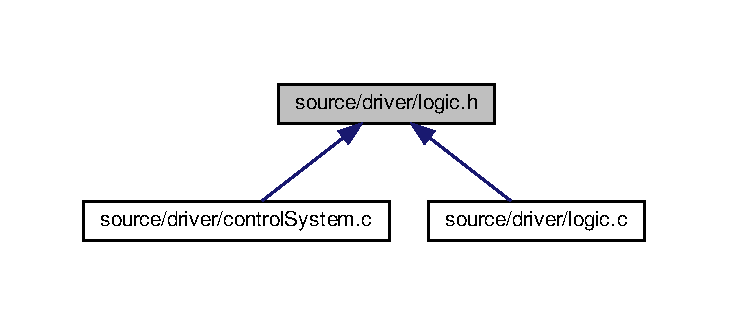
\includegraphics[width=350pt]{logic_8h__dep__incl}
\end{center}
\end{figure}
\subsection*{Functions}
\begin{DoxyCompactItemize}
\item 
void \hyperlink{logic_8h_a6f60f4629f53eeb7b91d70028f708227}{init\+Order\+System} (int $\ast$$\ast$order)
\begin{DoxyCompactList}\small\item\em Takes in an empty double array and fills it with default array values (0 and -\/1) \end{DoxyCompactList}\item 
void \hyperlink{logic_8h_aa2a5dd8ee4aa2ddfaaa0fa3ebaf99a59}{add\+Order} (int $\ast$$\ast$order)
\begin{DoxyCompactList}\small\item\em Loops through all buttons on each floor to check for orders. Adds order information to the order array. \end{DoxyCompactList}\end{DoxyCompactItemize}
\subsection*{Variables}
\begin{DoxyCompactItemize}
\item 
\mbox{\Hypertarget{logic_8h_a4a5c0ea05e5f03d798c2481965e1018d}\label{logic_8h_a4a5c0ea05e5f03d798c2481965e1018d}} 
int {\bfseries order} \mbox{[}10\mbox{]}\mbox{[}2\mbox{]}
\end{DoxyCompactItemize}


\subsection{Detailed Description}
Module that deals with order logic. 

\begin{DoxyAuthor}{Author}
Christian \& Ida 
\end{DoxyAuthor}
\begin{DoxyVersion}{Version}
0.\+1 
\end{DoxyVersion}
\begin{DoxyDate}{Date}
2022-\/02-\/25 
\end{DoxyDate}


\subsection{Function Documentation}
\mbox{\Hypertarget{logic_8h_aa2a5dd8ee4aa2ddfaaa0fa3ebaf99a59}\label{logic_8h_aa2a5dd8ee4aa2ddfaaa0fa3ebaf99a59}} 
\index{logic.\+h@{logic.\+h}!add\+Order@{add\+Order}}
\index{add\+Order@{add\+Order}!logic.\+h@{logic.\+h}}
\subsubsection{\texorpdfstring{add\+Order()}{addOrder()}}
{\footnotesize\ttfamily void add\+Order (\begin{DoxyParamCaption}\item[{int $\ast$$\ast$}]{order }\end{DoxyParamCaption})}



Loops through all buttons on each floor to check for orders. Adds order information to the order array. 


\begin{DoxyParams}[1]{Parameters}
\mbox{\tt in,out}  & {\em order} & A double array containing destination and direction of orders \\
\hline
\end{DoxyParams}


Definition at line 19 of file logic.\+c.

\mbox{\Hypertarget{logic_8h_a6f60f4629f53eeb7b91d70028f708227}\label{logic_8h_a6f60f4629f53eeb7b91d70028f708227}} 
\index{logic.\+h@{logic.\+h}!init\+Order\+System@{init\+Order\+System}}
\index{init\+Order\+System@{init\+Order\+System}!logic.\+h@{logic.\+h}}
\subsubsection{\texorpdfstring{init\+Order\+System()}{initOrderSystem()}}
{\footnotesize\ttfamily void init\+Order\+System (\begin{DoxyParamCaption}\item[{int $\ast$$\ast$}]{order }\end{DoxyParamCaption})}



Takes in an empty double array and fills it with default array values (0 and -\/1) 


\begin{DoxyParams}[1]{Parameters}
\mbox{\tt in,out}  & {\em order} & A double array containing destination and direction of orders \\
\hline
\end{DoxyParams}


Definition at line 6 of file logic.\+c.


\hypertarget{terminalUpdates_8h}{}\section{source/driver/terminal\+Updates.h File Reference}
\label{terminalUpdates_8h}\index{source/driver/terminal\+Updates.\+h@{source/driver/terminal\+Updates.\+h}}


Module for printing in terminal.  


{\ttfamily \#include \char`\"{}elevio.\+h\char`\"{}}\newline
Include dependency graph for terminal\+Updates.\+h\+:
\nopagebreak
\begin{figure}[H]
\begin{center}
\leavevmode
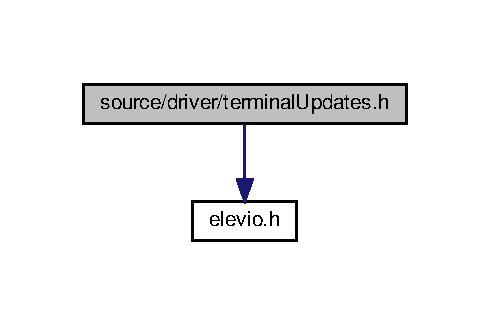
\includegraphics[width=235pt]{terminalUpdates_8h__incl}
\end{center}
\end{figure}
This graph shows which files directly or indirectly include this file\+:\nopagebreak
\begin{figure}[H]
\begin{center}
\leavevmode
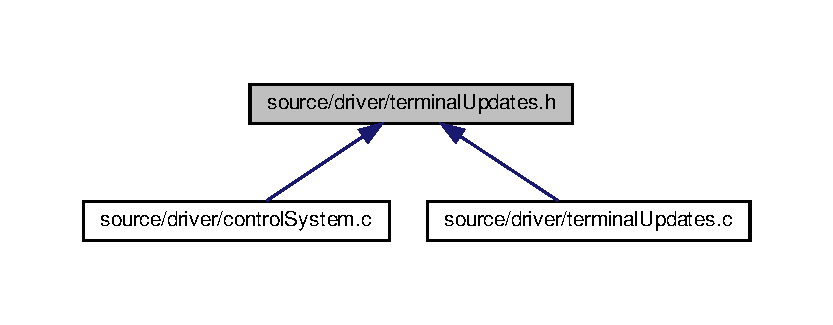
\includegraphics[width=350pt]{terminalUpdates_8h__dep__incl}
\end{center}
\end{figure}
\subsection*{Functions}
\begin{DoxyCompactItemize}
\item 
\mbox{\Hypertarget{terminalUpdates_8h_a6f3d029fddbaed9b098e49aa03c48c2b}\label{terminalUpdates_8h_a6f3d029fddbaed9b098e49aa03c48c2b}} 
void \hyperlink{terminalUpdates_8h_a6f3d029fddbaed9b098e49aa03c48c2b}{init\+Floor\+Update} ()
\begin{DoxyCompactList}\small\item\em Prints elevator initialization status. \end{DoxyCompactList}\item 
\mbox{\Hypertarget{terminalUpdates_8h_ae3cb7cca8ed1992d4136a1b7ef149650}\label{terminalUpdates_8h_ae3cb7cca8ed1992d4136a1b7ef149650}} 
void \hyperlink{terminalUpdates_8h_ae3cb7cca8ed1992d4136a1b7ef149650}{current\+Floor\+Update} ()
\begin{DoxyCompactList}\small\item\em Prints current elevator floor. \end{DoxyCompactList}\end{DoxyCompactItemize}


\subsection{Detailed Description}
Module for printing in terminal. 

\begin{DoxyAuthor}{Author}
Christian \& Ida 
\end{DoxyAuthor}
\begin{DoxyVersion}{Version}
0.\+1 
\end{DoxyVersion}
\begin{DoxyDate}{Date}
2022-\/02-\/25 
\end{DoxyDate}

%--- End generated contents ---

% Index
\backmatter
\newpage
\phantomsection
\clearemptydoublepage
\addcontentsline{toc}{chapter}{Index}
\printindex

\end{document}
